\documentclass[a4paper]{article}

\usepackage[utf8]{inputenc}
\usepackage[T1]{fontenc}
\usepackage{graphicx}
\usepackage[frenchb]{babel}
\usepackage{amsmath}
\usepackage{listings}

% define our color
\usepackage{xcolor}

% code color
\definecolor{ligthyellow}{RGB}{250,247,220}
\definecolor{darkblue}{RGB}{5,10,85}
\definecolor{ligthblue}{RGB}{1,147,128}
\definecolor{darkgreen}{RGB}{8,120,51}
\definecolor{darkred}{RGB}{160,0,0}

% other color
\definecolor{ivi}{RGB}{141,107,185}


\lstset{
    language=scilab,
    captionpos=b,
    extendedchars=true,
    frame=lines,
    numbers=left,
    numberstyle=\tiny,
    numbersep=5pt,
    keepspaces=true,
    breaklines=true,
    showspaces=false,
    showstringspaces=false,
    breakatwhitespace=false,
    stepnumber=1,
    showtabs=false,
    tabsize=3,
    basicstyle=\small\ttfamily,
    backgroundcolor=\color{ligthyellow},
    keywordstyle=\color{ligthblue},
    morekeywords={include, printf, uchar},
    identifierstyle=\color{darkblue},
    commentstyle=\color{darkgreen},
    stringstyle=\color{darkred},
}

\begin{document}

\title{VISA -- TP Couleurs}
\author{Arnaud Cojez}
\date{mardi 7 novembre 2016}

\maketitle

\newpage
\tableofcontents
\newpage
%----------------------------------------------------------------------------------------
%	INTRODUCTION
%----------------------------------------------------------------------------------------

\section{Introduction}
Une fois la capture de la lumière maîtrisée, il nous faut définir la façon dont sera stockée l'image formée.\\
L'information des pixels d'une image peut être stockée selon différentes représentations. Par exemple, nous pouvons considérer différentes couleurs comme les composantes de l'image.\\
Ainsi, chaque opération effectuée sur une image aura un effet lié à la représentation de celle-ci.\\

Le long de ce TP, nous utiliserons l'espace de couleurs HSB (Hue-Saturation-Brightness). Celui-ci nous permet de modifier la luminance, la teinte et la saturation de l'image.\\
Les fichiers utilisés sont des images composant le test d'Ishihara, qui permet de détecter les déficiences dichromatiques telles que le daltonisme.

\begin{figure}[h]
\begin{center}
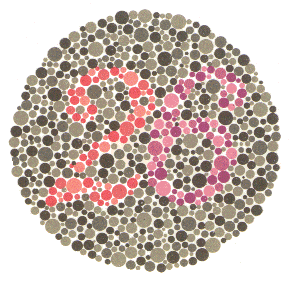
\includegraphics[width=170px]{planche_26.png}
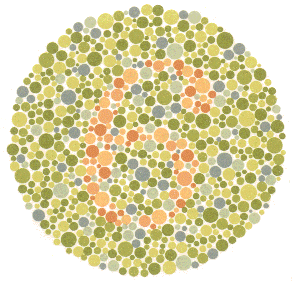
\includegraphics[width=170px]{planche_6.png}
\end{center}
\caption{Planches issues du Test d'Ishihara}
\end{figure}


\clearpage
%----------------------------------------------------------------------------------------
%	MANIPULATION DE LA LUMINANCE
%----------------------------------------------------------------------------------------

\section{Manipulation de la luminance}

\clearpage
%----------------------------------------------------------------------------------------
% RÉTABLISSEMENT DE LA SATURATION
%----------------------------------------------------------------------------------------

\section{Rétablissement de la saturation}

\clearpage
%----------------------------------------------------------------------------------------
%	TRANSFORMATION DE LA TEINTE
%----------------------------------------------------------------------------------------

\section{Transformation de la teinte}

\clearpage

%----------------------------------------------------------------------------------------
%	ANALYSE DANS DES ESPACES COULEURS ADAPTÉS
%----------------------------------------------------------------------------------------

\section{Analyse dans des espaces couleur adaptés}

\clearpage
%----------------------------------------------------------------------------------------
%	MODIFICATION DE LA LUMINANCE ADAPTÉE
%----------------------------------------------------------------------------------------

\section{Modification de la luminance adaptée}

\clearpage
%----------------------------------------------------------------------------------------

%----------------------------------------------------------------------------------------
%	CONCLUSION
%----------------------------------------------------------------------------------------

\section{Conclusion}
Nous avons pu constater qu'une image possède plusieurs composantes, mais que celles-ci peuvent différer en fonction de la représentation de l'image, ou espace colorimétrique.\\

Chaque opération sur un espace colorimétrique aura un effet propre à l'espace. De plus, les jeux de composantes pourront mettre en évidence différents phénomènes apparaissant sur l'image.\\
Il existe cependant une limite aux opérations sur les espaces colorimétriques. Lorsqu'une image a été modifiée, il est possible de perdre de l'information à cause d'un effet de plancher/plafond.\\

Il peut donc être utile de convertir un espace colorimétrique en un autre afin de pouvoir profiter d'opérations spécifiques, ou pour analyser la composition de l'image sous un autre angle.

\clearpage
%----------------------------------------------------------------------------------------

\section{Annexe}

\end{document}
